\section{Estimation, Evaluation and Simulation procedure} \label{sec:estimation-evaluation-simulation}

This section presents computational aspects of the estimation, such as presenting the mathematical programming formulation of both the linear and the nonparametric models, presenting the evaluation metric and the cross-validation methodology
%, which is essential in the process of building the function $\hat{Q}_{y_\tau|X}(\alpha)$.
and the simulation procedure to produce future scenarios of Wind Power.
The methodology is implemented in R and Julia languages (relying heavily on the packages JuMP, Gurobi, RCall and Dierckx) and using the Gurobi solver. 

\subsection{Estimating the QRAL model}

The QRAL model, as described in problem (\ref{eq:adalasso_model_mat1})-(\ref{eq:adalasso_model_mat2}), can be implemented as a linear programming problem as shown below:
\begin{IEEEeqnarray}{lr}
	\underset{\beta_{0},\beta,\varepsilon_{t j}^{+},\varepsilon_{t j}^{-}}{\text{min}} \sum_{j \in J} \sum_{t \in T}(\alpha_j\varepsilon_{t j}^{+}+(1-\alpha_j)\varepsilon_{t j}^{-}) \span \nonumber  \\
	\span + \lambda \sum_{p \in P} \sum_{j \in J} w_{pj} (\xi^+_{pj} + \xi^-_{pj}) \nonumber \\ 
	\span + \gamma \sum_{p \in P} \sum_{j \in J'} (D2_{pj}^+ + D2_{pj}^-),  \label{eq:adalasso-1} \\
	\mbox{subject to:} \nonumber & \\
	\varepsilon_{t j}^{+}-\varepsilon_{t j}^{-}=y_{t}-\beta_{0 j}-\beta_{j}^T x_{t},& \forall t \in T ,\forall j \in J,\\
	\xi_{pj}^+ - \xi_{pj}^- = \beta_{pj},&\forall p \in P, \forall j \in J\\ 
	D2_{pj}^+ - D2_{pj}^- = \frac{\left(\frac{\beta_{p,j+1}-\beta_{pj}}{\alpha_{j+1}-\alpha_{j}}\right)-\left(\frac{\beta_{p,j}-\beta_{p,j-1}}{\alpha_{j}-\alpha_{j-1}}\right)}{\alpha_{j+1}-\alpha_{j-1}}, \span   \nonumber \\
	\span \forall p\in P, \forall j \in J',  \\
	\beta_{0j} + \beta_{j}^T x_{t} \leq \beta_{0,j+1} + \beta_{j+1}^T x_{t},&\forall t \in T, \forall j \in J_{(-1)}, \label{eq:qral-crossing} \\
	\varepsilon_{t j}^{+},\varepsilon_{t j}^{-}\geq0,&\forall t \in T, \forall j \in J,\\
	\xi_{pj}^+, \xi_{pj}^- \geq 0, & \forall p\in P, \forall j \in J, \\
	D2_{pj}^+, D2_{pj}^- \geq 0, & \forall p\in P, \forall j \in J', \label{eq:adalasso-ult} 
\end{IEEEeqnarray}
where $J_{(-1)} = \{ 2, \dots, |J| \}$ is the set which contains all indexes but the first and $J'  = \{ 2, \dots, |J|-1 \}$ is the set which contains all indexes but the first and the last.
Variables $\varepsilon^+_t$ and $\varepsilon^-_t$ represent the quantities $|y-q(\cdot)|^+$ and $|y-q(\cdot)|^-$, respectively. The first line on the objective function represents the sum of the check function over all $j$: $ \rho_{\alpha_j}(y-q(\cdot)) = \alpha_j \varepsilon^+_{tj} + (1-\alpha_j) \varepsilon^-_{tj}$. The constraint (\ref{eq:qral-crossing}) assures that the quantile function be monotonic by forcing that, for every $x_t$ and $\alpha_j$-quantile, $q_{\alpha_{j}}(x_t) \leq q_{\alpha_{j+1}}(x_t)$.
The second derivative term $D^2_{\alpha_j}\beta_j$ is implemented on the optimization problem by adding a penalty on the objective function to penalize its absolute value, modeled as the sum of auxiliary variables $D2_{pj}^+ + D2_{pj}^-$. The tuning parameter $\gamma$ controls how rough the sequence $\{\beta_{pj}\}_{j \in J}$ can be, for a given $p$.

\subsection{Evaluation Metric}

In this section, we present the metric for which the model fit can be evaluated. From this metric, we show two different forms - information criteria and cross validation - to determine the best tuning parameters $\lambda$ and $\gamma$.

In order to evaluate our predictions, we need to define an error metric. The minimization of this error metric is the objective in estimating the statistical model. 
As conditional distribution is the focus in this paper, we use a performance measurement which emphasizes the correctness across quantiles. Depending on the application, it might be interesting to put different weights on different quantiles. In this work, however, we will treat every quantile as equals concerning the error measure.
The chosen error function is the Mean Absolute Percentage Error (MAPE), defined by
\begin{equation}
MAPE_{\lambda,\gamma}= \frac{1}{|J|} \frac{1}{|T|}  \sum_{t \in T} \sum_{j \in J} \left| \frac{q_t^{\alpha_{j}}- \hat q_t^{\alpha_{j}}}{q_t^{\alpha_{j}}}  \right|. 
\end{equation}
where $q_t^{\alpha_{j}}$ is the $\alpha$-quantile from the data (in the case study, we use the monthly distribution as a good enough approximation of the true quantile, as RG series such as wind power are stationary) and $\hat q_t^{\alpha_j}$ is the $\alpha$-quantile from these scenarios, when estimating the model with parameters $\lambda$ and $\gamma$.
This function has the advantage of penalizing error proportionally to the quantile value it is estimating. 


\subsection{Time-series Cross Validation} \label{sec:cv}

Estimating the QRAL involves parameters $\lambda$ and $\gamma$, which should be known \textit{a priori}. In statistics and machine learning, a popular technique is using cross-validation (CV) to select the best value of parameters from the range of possibilities. How to select their values among this range is a crucial point in our methodology, as the estimated coefficients vary considerably with respect to parameter choice.

Out of the different possible implementations of CV, we use the $\mathcal{K}$-fold CV. It consists in first partitioning the dataset in $\mathcal{K}$ equally sized sets, which are the $\mathcal{K}$ folds. For each fold $k \in \{1,\dots,\mathcal{K}\}$, the remaining $\mathcal{K}-1$ folds are used to estimate the model using parameter $\theta$ (for the QRAL model, $\theta = [\gamma \quad \lambda]^T$) and predicting the values in fold $k$. The error function $MAPE_\theta$ measures the result of this prediction.
So, the CV error is given by the sum of all folds, for a given model which uses the vector of parameter $\theta$ is given by
\[
 CV(\theta) = \sum_{k \in \mathcal{K}} \sum_{j \in J} MAPE_\theta.\label{eq:cv-error}
\]
The optimum parameter $\theta^*_{CV}$, according to this methodology, is the value of $\theta$ which minimizes the CV error
\begin{equation}
\theta_{CV}^* = \argmin_\theta CV(\theta) .\label{eq:cv-equation}
\end{equation}

The usage of CV is not straightforward when data is dependent, which is the case of time series. As it is time dependent, one can be interested in using either all observations or to take the dependence away to not interfere on the estimation. The works
\cite{bergmeir_note_2017} and \cite{bergmeir_use_2012} deals specifically with the usage of CV in a time series context. They provide tests with both $\mathcal{K}$-fold CV and $\mathcal{K}$-fold with non-dependent data. Both schemes are shown of Figure \ref{fig:cross-validation-scheme}.
\begin{figure}
	\centering
	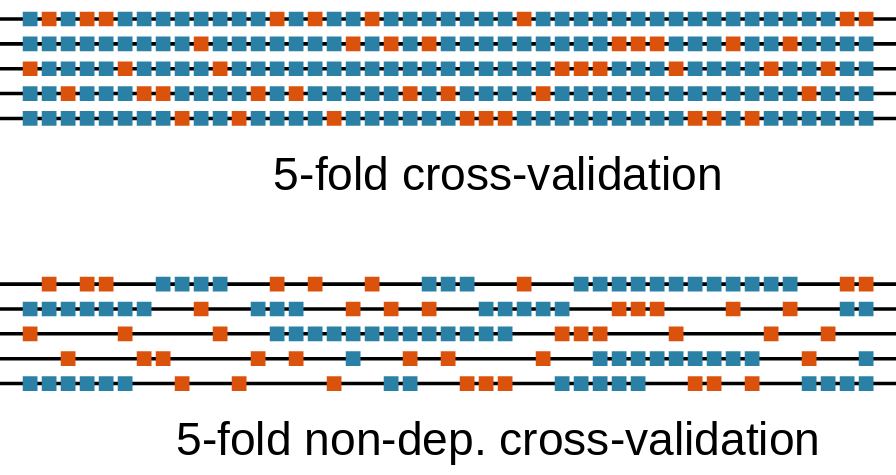
\includegraphics[width=0.7\linewidth]{Images/Cross-validation-scheme}
	\caption{$\mathcal{K}$-fold CV and $\mathcal{K}$-fold with non-dependent data. Observations in blue are used to estimation and in orange for evaluation. Note that non-dependent data does not use all dataset in each fold. Image from \cite{bergmeir_note_2017}.}
	\label{fig:cross-validation-scheme}
\end{figure}
In both settings, the training data is randomly split into a collection of sets $S_k$, forming a $\mathcal{K}$ size partition. Each of these $S_k$ is used as test set, while the rest is used to estimate coefficients which will be used to predict values of $S_k$. 
As there are $\mathcal{K}$ folds, this procedure is done $\mathcal{K}$ times. 
So, for a given vector of tuning parameter $\theta$, the CV score is given by the sum of the error function for each fold. 
As the CV score is nonconvex, the optimization in (\ref{eq:cv-equation}) is done by iterating over a sequence of values in a thin grid and choosing the smallest one.




\subsection{Information Criteria for Quantile Regression}
Using CV can be computationally expensive, as the full estimation is done several times for each tuning parameter - in this case, $\gamma$ and $\lambda$. Other form of deciding the quantity of variables that provides a good equilibrium between in-sample prediction and parsimony is the Information Criteria.

Information criteria summarizes two aspects. One of them refers to how well the model fits the in-sample observations and the other part penalizes the quantity of covariates used in the model. By penalizing how big our model is, we prevent overfitting from happening. So, in order for a covariate to be included in the model, it must supply enough goodness of fit.
In \cite{machado1993robust}, it is presented a variation of the Schwarz criteria for M-estimators that includes quantile regression. The Schwarz Information Criteria (SIC), adapted to the quantile autoregression case, is presented below:
{\small
\begin{align} 
\begin{split}
SIC_m = \sum_{j \in J} \left( \log \left(\sum_{t \in T}\rho_{\alpha_j}(y_t - \beta_{0j} - \beta_j^T x_t) \right) +  \frac{\log|T||\epsilon_j|}{2|T|}  \right),\label{eq:SIC}
\end{split}					
\end{align}}
where $K(m)$ is the quantity of coefficients $\beta_{pj}$ greater than zero in the model $m$.
By minimizing the $SIC$ function, the chosen model is the one with the best combination, according to this metric, of fit and parsimony among all models. 

Even though CV is very popular and produce great results, selecting model with Information Criteria involves less computational time. For the case where the selected model is very similar, it might be the case that the estimation methodology may change a little bit. It is definitely a topic that worths researching.


% \todoi{Ver se novas figuras (R/grafico-cv.r) e ver se incluir outras formas de CV} % escolhemos trabalhar apenas com este tipo de CV





\subsection{Scenario generation} \label{sec:scenario-generation}

This section presents how to generate future scenarios of time series $y_t$ from the estimated coefficients from a QR model. 
%Let $|T|$ be the total length of $\{y_t\}$ and $S$ the number of scenarios of size $K$ we produce. 
%The variables chosen to compose $x_t$ can be either exogenous variables, autoregressive components of $y_t$ or both. We use a nonparametric approach which to estimate, at every $t$, the $k$-step ahead conditional density of $y_t$.
To produce $S$ different future scenarios $\{ \hat{y}_{\tau,s} \}_{\tau=|T|+1}^{|T|+K}$, we use the following procedure:

\noindent\rule{\columnwidth}{3pt}

Procedure for simulating $S$ future scenarios of $\{y_{\tau,s}\}$

\noindent\rule{\columnwidth}{1pt}

\begin{enumerate}
	
	\item Estimate the QR model solving the QRAL optimization problem defined in equation (\ref{eq:adalasso-1})-(\ref{eq:adalasso-ult}). 
	A sequence of coefficients $\{ \hat\beta_{0j} \}_{j \in J}$ and $\{ \hat\beta_{j} \}_{j \in J}$ are the output from this problem. 

	\item Initialize time index $\tau = |T| + 1$.
	
	\item For each scenario $s \in S$, do:
		\begin{enumerate}

		\item Let $x_{\tau,s} = [y_{\tau-1,s}, \dots, y_{\tau-12,s}]$ be the vector of explanatory variables used as input to predict the conditional distribution function in time $\tau$ and scenario $s$.

		\item Let $\tilde{Q}_{y_{\tau,s}|X}:A \times \mathbb{R}^d \rightarrow \mathbb{R}$ be the discrete quantile function. Its values are mapped according to the estimated quantile $\tilde Q_{y_{\tau,s}|X}(\alpha_j, x_{\tau,s}) \leftarrow \hat\beta_{0j} + \hat\beta_j^T x_{\tau,s}$, for all $j \in J$.
		
		\item In order to define the continuous function $\hat{Q}_{y_{\tau,s}|X}:[0,1] \times \mathbb{R}^d \rightarrow \mathbb{R}$ from $\tilde Q_{y_{\tau,s}|X}$, use linear interpolation connecting the points. As $0 < \alpha_1 < \cdots < \alpha_{|J|} < 1$, there are no quantile estimates for the intervals $[0,\alpha_1]$ and $[\alpha_{|J|},1]$. These gaps are filled by linearly extending the line that connects $\alpha_1$ to $\alpha_2$ on the left hand side and extending the line that connects $\alpha_{|J|-1}$ to $\alpha_{|J|}$ on the right hand side until the support $[0,1]$ is fully mapped.  

		% \item In any given period $\tau$, for every $\alpha \in A$, we estimate $q_{\alpha_{j}}$, for every $j \in J$.
		% Note that $x_{\tau}$ is supposed to be known at time $\tau$\footnote{In the presence of exogenous variables that are unknown, it is advisable to incorporate its uncertainty by considering different scenarios. In each scenario, though, $x_{\tau}$ must be considered fully known.}.
		
		% \item Let $\hat{Q}_{y_{\tau,s}|X}(\alpha,x_\tau)$ be the estimated quantile function of ${y}_{\tau,s}$. 
		% At first, we define a discrete quantile function $\tilde{Q}_{y_{\tau,s}}$. By mapping every $\alpha \in A$ with its estimated quantile $\hat{q}_{\alpha_j}(x_t)$, we define function $\tilde{Q}_{y_{\tau,s}}$. In order to produce a continuous function from a set of ordered points, we use linear interpolation and we arrive on the Quantile function $\hat{Q}_{y_{\tau}}$.
		
		%This process is described in more details on section \ref{sec:estimating-distribution}. 
		\item Let $U$ be a random variable with uniform distribution over the interval $[0,1]$. By using the result of the probability integral transform (PIT), random variable $F^{-1}_{y_{\tau,s}}(U)$ has the same distribution as $y_{\tau,s}$. The value of $y_{\tau,s}$ is built by drawing one random observation of U and applying the PIT.

		 \end{enumerate}
	% let $x_{\tau,s} = [y_{\tau-1,s}, \dots, y_{\tau-12,s}]$ be the vector of explanatory variables, used as input to predict the conditional distribution function in time $\tau$ and scenario $s$.
	
	
	\item Let $\tau = \tau + 1$. If $\tau > K$, then stop. Else, go back to step 3) . 


\end{enumerate}


\noindent\rule{\columnwidth}{1pt}